\hypertarget{photosynthesis-and-cellular-respiration}{%
\chapter{Photosynthesis And Cellular Respiration}\label{photosynthesis-and-cellular-respiration}}

Plants acquire energy from sunlight through photosynthesis. Animals get their energy by breaking down chemical bonds in nutrients during cellular respiration. In eukaryiotic cells, photosynthesis happens in chloroplasts, cellular respiration in mitochondria. In both photosynthesis and cellular respiration, ATP production involves an electron transfer chain and chemiosmosis.



\begin{figure}

{\centering 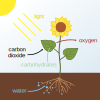
\includegraphics[width=0.7\linewidth]{./figures/photosynthesis/Photosynthesis_en} 

}

\caption{\href{https://commons.wikimedia.org/wiki/File:Photosynthesis_en.svg}{Schematic of photosynthesis in plants. The carbohydrates produced are stored in or used by the plant which in turn may provide food for heterotrophic organims such as animals.}}\label{fig:photosynthesispic}
\end{figure}

\hypertarget{the-electron-transport-chain-and-chemiosmosis}{%
\section{The Electron Transport Chain And Chemiosmosis}\label{the-electron-transport-chain-and-chemiosmosis}}

The electron transport chain (ETC) is a series of complexes that transfer electrons from electron donors to electron acceptors via redox (both reduction and oxidation occurring simultaneously) reactions, and couples this electron transfer with the transfer of protons (H\textsuperscript{+} ions) across a membrane. The electron transport chain is built up of peptides, enzymes, and other molecules.

The flow of electrons through the electron transport chain is an exergonic process. The energy from the redox reactions create an electrochemical proton gradient that drives the synthesis of adenosine triphosphate (ATP). In aerobic respiration, the flow of electrons terminates with molecular oxygen being the final electron acceptor. In anaerobic respiration, other organic or inorganic electron acceptors are used, such as lactic acid and sulfate, for example.

In the electron transport chain, the redox reactions are driven by the Gibbs free energy state of the components. Gibbs free energy is related to a quantity called the redox potential. The complexes in the electron transport chain harvest the energy of the redox reactions that occur when transferring electrons from a low redox potential to a higher redox potential, creating an electrochemical gradient. It is the electrochemical gradient created that drives the synthesis of ATP via coupling with oxidative phosphorylation with ATP synthase.

The electron transport chain, and site of oxidative phosphorylation is found on the inner mitochondrial membrane. The energy stored from the process of respiration in reduced compounds (such as NADH and FADH) is used by the electron transport chain to pump protons into the inter membrane space, generating the electrochemical gradient over the inner mitochrondrial membrane.



\begin{figure}

{\centering \includegraphics[width=0.7\linewidth]{./figures/photosynthesis/Mitochondrial_electron_transport_chain—Etc4} 

}

\caption{\href{https://commons.wikimedia.org/wiki/File:Mitochondrial_electron_transport_chain—Etc4.svg}{The electron transport chain} in the mitochondrion is the site of oxidative phosphorylation in eukaryotes. The NADH and succinate generated in the citric acid cycle are oxidized, providing energy to power ATP synthase.}\label{fig:electrontransfer}
\end{figure}

In photosynthetic eukaryotes, the electron transport chain is found on the thylakoid membrane. Here, light energy drives the reduction of components of the electron transport chain and therefore causes subsequent synthesis of ATP. The electron transport chain, and site of oxidative phosphorylation is found on the inner mitochondrial membrane. The energy stored from the process of respiration in reduced compounds (such as NADH and FADH) is used by the electron transport chain to pump protons into the inter membrane space, generating the electrochemical gradient over the inner mitochrondrial membrane.

Hydrogen ions, or protons, will diffuse from an area of high proton concentration to an area of lower proton concentration, and an electrochemical concentration gradient of protons across a membrane can be harnessed to make ATP. This process is related to osmosis, the diffusion of water across a membrane, which is why it is called ``chemiosmosis''.

The formation of adenosine triphosphate (ATP) by the movement of hydrogen ions (H\textsuperscript{+}) across a membrane during cellular respiration or photosynthesis is an example of chemiosmosis. ATP synthase is the enzyme that makes ATP by chemiosmosis. It allows protons to pass through the membrane and uses the free energy difference to phosphorylate adenosine diphosphate (ADP), making ATP. The generation of ATP by chemiosmosis occurs in mitochondria and chloroplasts, as well as in most bacteria and archaea, an electron transport chain pumps H\textsuperscript{+} ions in the thylakoid spaces through thylakoid membranes to stroma (fluid). The energy from the electron movement through electron transport chains cross through ATP synthase which allows the proton to pass through them and use this free energy difference to photophosphorylate ADP making ATP.

\hypertarget{photosynthesis}{%
\section{Photosynthesis}\label{photosynthesis}}

Photosynthesis is a process used by plants and other organisms to convert light energy into chemical energy that can later be released to fuel the organisms' activities. This chemical energy is stored in carbohydrate molecules, such as sugars, which are synthesized from carbon dioxide and water -- hence the name photosynthesis, from the Greek phōs (φῶς), ``light'', and sunthesis (σύνθεσις), ``putting together''. In most cases, oxygen is also released as a waste product. Most plants, most algae, and cyanobacteria perform photosynthesis; such organisms are called photoautotrophs. Photosynthesis is largely responsible for producing and maintaining the oxygen content of the Earth's atmosphere, and supplies most of the energy necessary for life on Earth.



\begin{figure}

{\centering 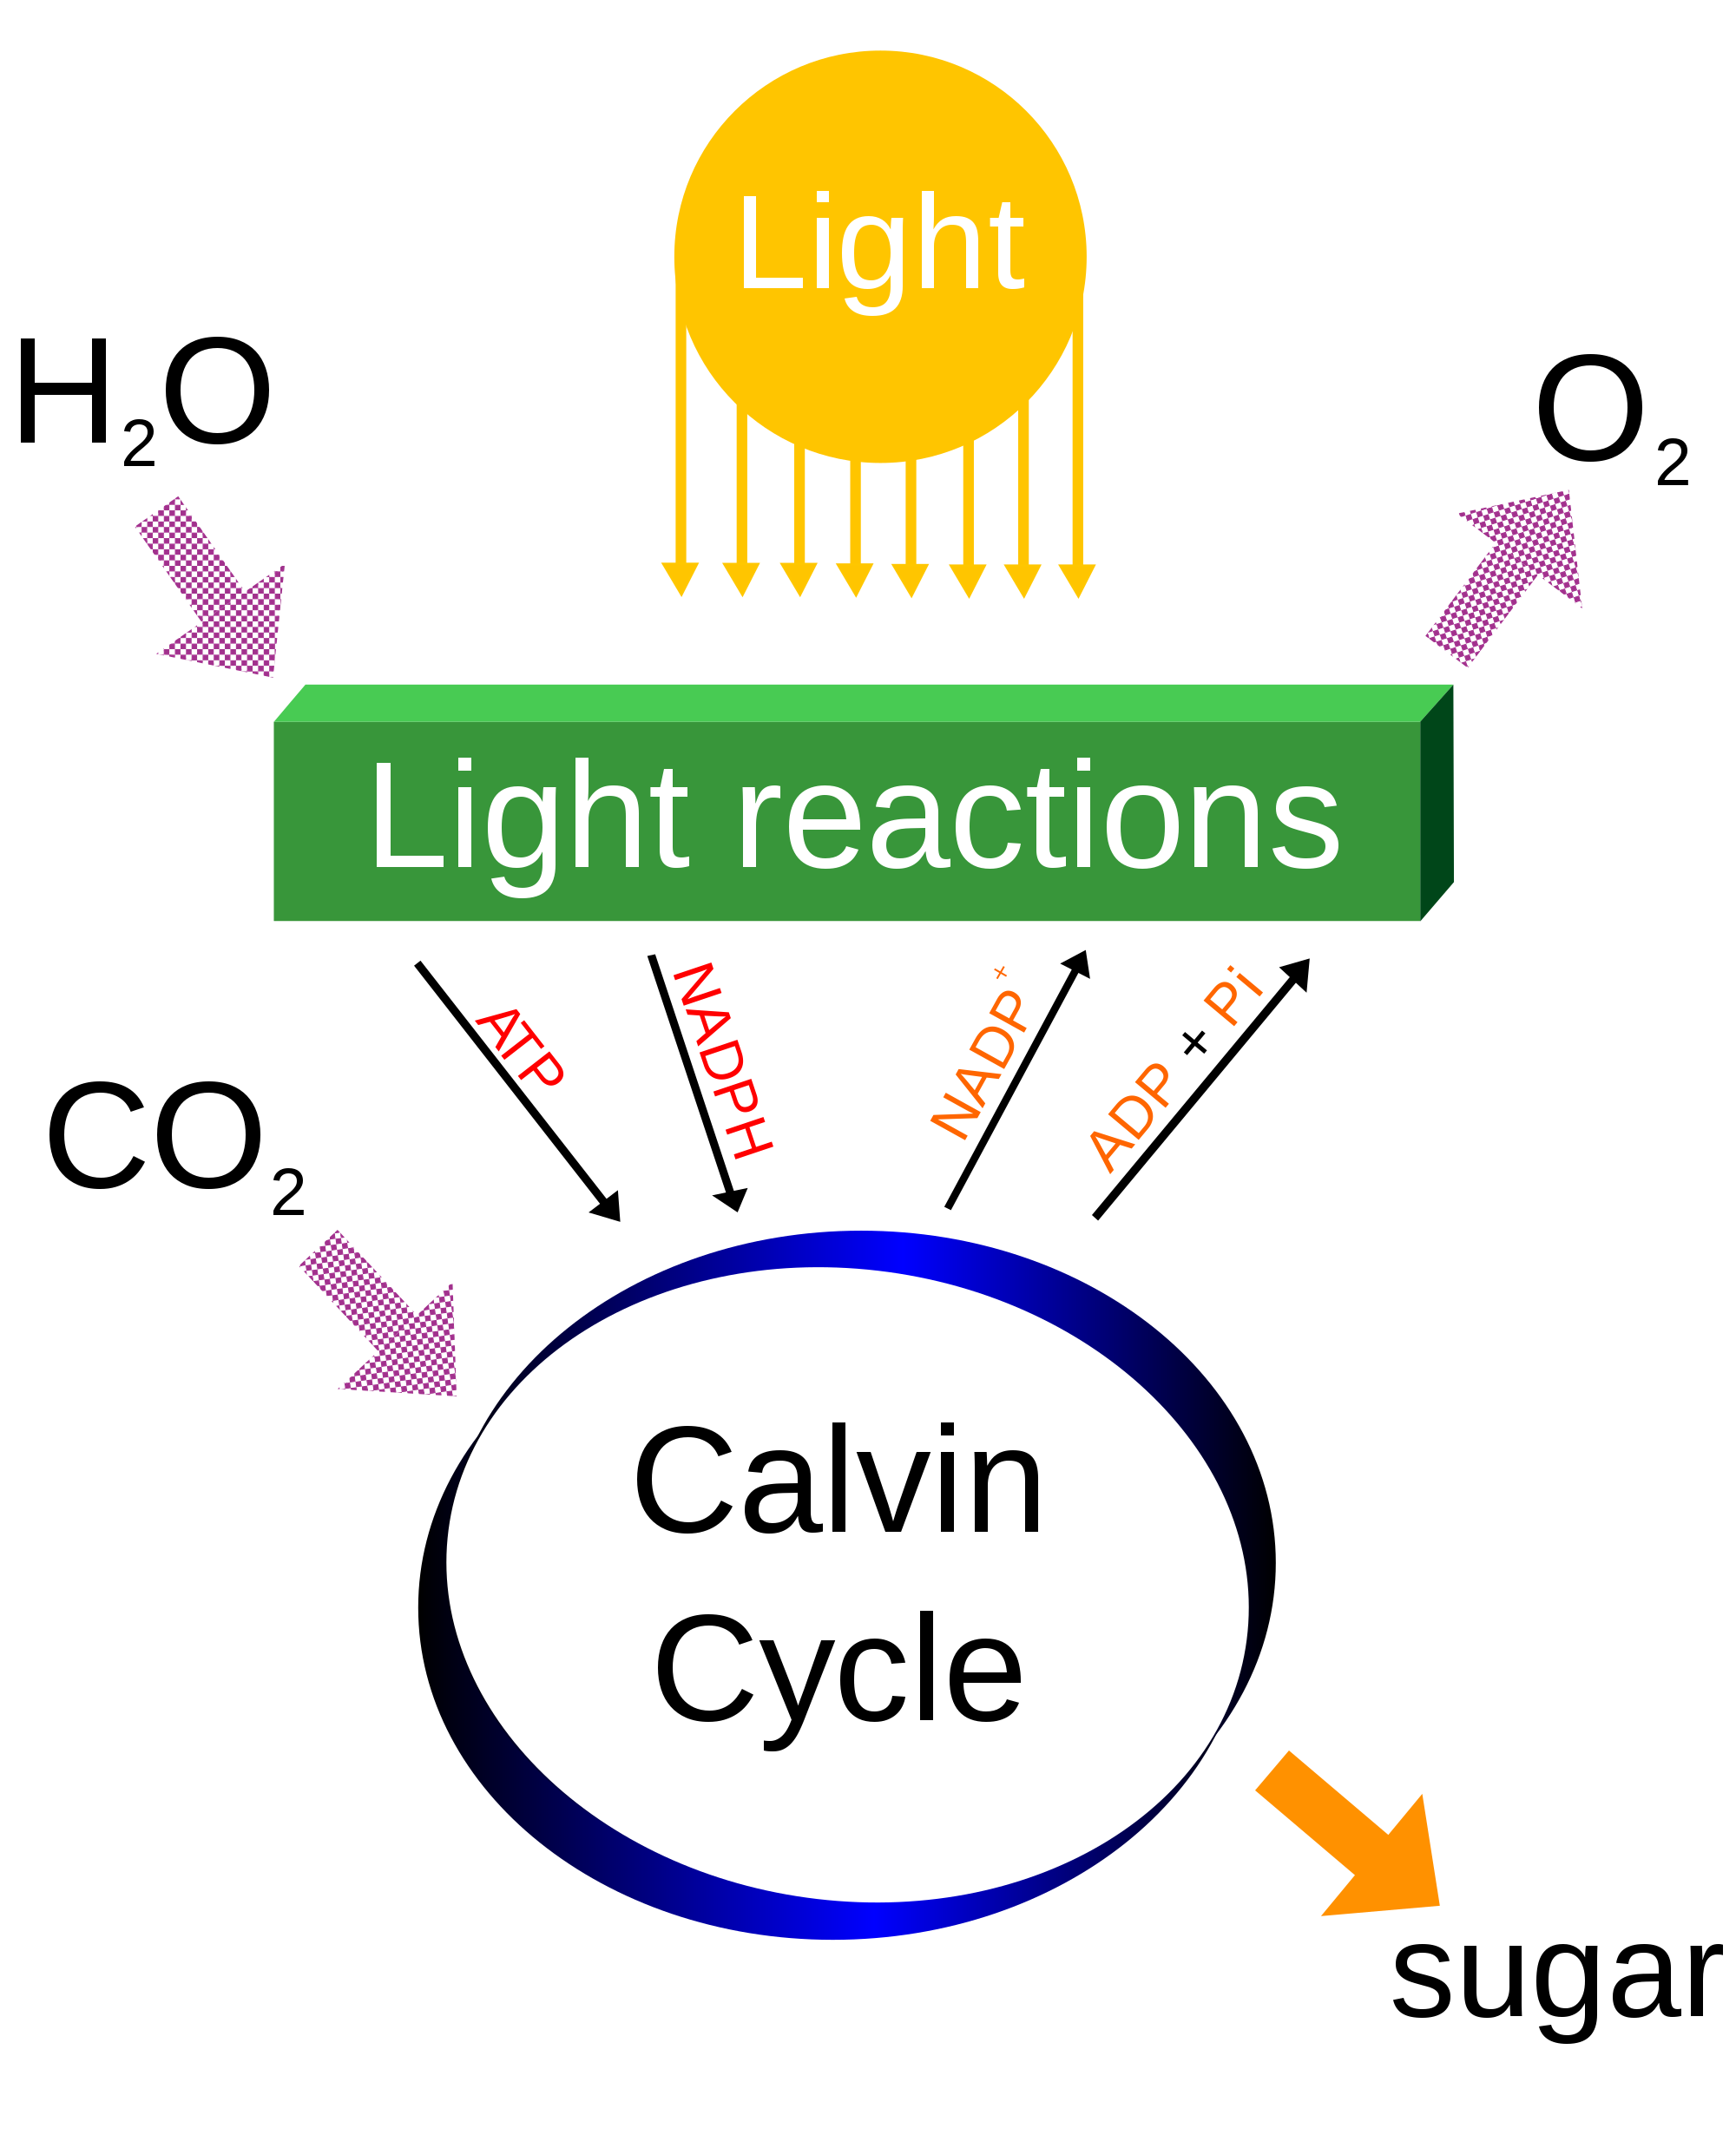
\includegraphics[width=0.7\linewidth]{./figures/photosynthesis/Simple_photosynthesis_overview} 

}

\caption{\href{https://commons.wikimedia.org/wiki/File:Simple_photosynthesis_overview.svg}{Photosynthesis changes sunlight into chemical energy, splits water to liberate O2, and fixes CO\textsubscript{2} into sugar.}}(\#fig:simplephotooverview )
\end{figure}

Although photosynthesis is performed differently by different species, the process always begins when energy from light is absorbed by proteins called reaction centres that contain green chlorophyll pigments. In plants, these proteins are held inside organelles called chloroplasts, which are most abundant in leaf cells, while in bacteria they are embedded in the plasma membrane. In these light-dependent reactions, some energy is used to strip electrons from suitable substances, such as water, producing oxygen gas. The hydrogen freed by the splitting of water is used in the creation of two further compounds that serve as short-term stores of energy, enabling its transfer to drive other reactions: these compounds are reduced nicotinamide adenine dinucleotide phosphate (NADPH) and adenosine triphosphate (ATP), the ``energy currency'' of cells.



\begin{figure}

{\centering 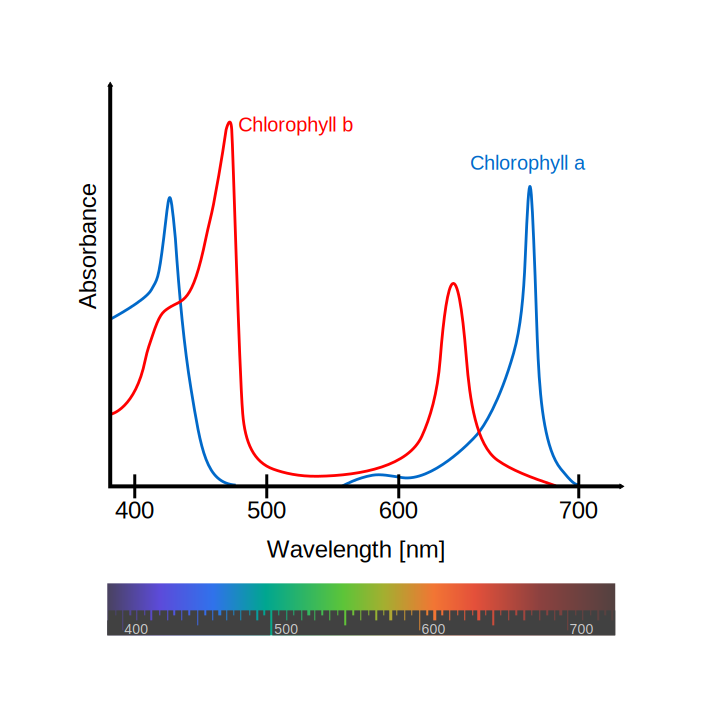
\includegraphics[width=0.7\linewidth]{./figures/photosynthesis/Chlorophyll_ab_spectra-en} 

}

\caption{\href{https://commons.wikimedia.org/wiki/File:Chlorophyll_ab_spectra-en.svg}{Absorbance spectra of free chlorophyll} a (blue) and b (red) in a solvent. The action spectra of chlorophyll molecules are slightly modified in vivo depending on specific pigment--protein interactions.}\label{fig:chlorophylspectra}
\end{figure}

In plants, algae and cyanobacteria, long-term energy storage in the form of sugars is produced by a subsequent sequence of light-independent reactions called the Calvin cycle; some bacteria use different mechanisms, such as the reverse Krebs cycle, to achieve the same end. In the Calvin cycle, atmospheric carbon dioxide is incorporated into already existing organic carbon compounds, such as ribulose bisphosphate (RuBP). Using the ATP and NADPH produced by the light-dependent reactions, the resulting compounds are then reduced and removed to form further carbohydrates, such as glucose.

The first photosynthetic organisms probably evolved early in the evolutionary history of life and most likely used reducing agents such as hydrogen or hydrogen sulfide, rather than water, as sources of electrons. Cyanobacteria appeared later; the excess oxygen they produced contributed directly to the oxygenation of the Earth, which rendered the evolution of complex life possible. Today, the average rate of energy capture by photosynthesis globally is approximately 130 terawatts, which is about eight times the current power consumption of human civilization. Photosynthetic organisms also convert around 100--115 billion tons (91-104 petagrams) of carbon into biomass per year.

Photosynthetic organisms are photoautotrophs, which means that they are able to synthesize food directly from carbon dioxide and water using energy from light. However, not all organisms use carbon dioxide as a source of carbon atoms to carry out photosynthesis; photoheterotrophs use organic compounds, rather than carbon dioxide, as a source of carbon. In plants, algae, and cyanobacteria, photosynthesis releases oxygen. This is called oxygenic photosynthesis and is by far the most common type of photosynthesis used by living organisms. Although there are some differences between oxygenic photosynthesis in plants, algae, and cyanobacteria, the overall process is quite similar in these organisms. There are also many varieties of anoxygenic photosynthesis, used mostly by certain types of bacteria, which consume carbon dioxide but do not release oxygen.

Carbon dioxide is converted into sugars in a process called carbon fixation; photosynthesis captures energy from sunlight to convert carbon dioxide into carbohydrate. Carbon fixation is an endothermic redox reaction. In general outline, photosynthesis is the opposite of cellular respiration: while photosynthesis is a process of reduction of carbon dioxide to carbohydrate, cellular respiration is the oxidation of carbohydrate or other nutrients to carbon dioxide. Nutrients used in cellular respiration include carbohydrates, amino acids and fatty acids. These nutrients are oxidized to produce carbon dioxide and water, and to release chemical energy to drive the organism's metabolism. Photosynthesis and cellular respiration are distinct processes, as they take place through different sequences of chemical reactions and in different cellular compartments.

Photosynthesis occurs in two stages. In the first stage, light-dependent reactions or light reactions capture the energy of light and use it to make the energy-storage molecules ATP and NADPH. During the second stage, the light-independent reactions use these products to capture and reduce carbon dioxide.

Most organisms that utilize oxygenic photosynthesis use visible light for the light-dependent reactions, although at least three use shortwave infrared or, more specifically, far-red radiation.

Some organisms employ even more radical variants of photosynthesis. Some archaea use a simpler method that employs a pigment similar to those used for vision in animals. The bacteriorhodopsin changes its configuration in response to sunlight, acting as a proton pump. This produces a proton gradient more directly, which is then converted to chemical energy. The process does not involve carbon dioxide fixation and does not release oxygen, and seems to have evolved separately from the more common types of photosynthesis.

\hypertarget{photosynthetic-membranes-and-organelles}{%
\subsection{Photosynthetic Membranes And Organelles}\label{photosynthetic-membranes-and-organelles}}

In photosynthetic bacteria, the proteins that gather light for photosynthesis are embedded in cell membranes. In its simplest form, this involves the membrane surrounding the cell itself. However, the membrane may be tightly folded into cylindrical sheets called thylakoids, or bunched up into round vesicles called intracytoplasmic membranes. These structures can fill most of the interior of a cell, giving the membrane a very large surface area and therefore increasing the amount of light that the bacteria can absorb.

In plants and algae, photosynthesis takes place in organelles called chloroplasts. A typical plant cell contains about 10 to 100 chloroplasts. The chloroplast is enclosed by a membrane. This membrane is composed of a phospholipid inner membrane, a phospholipid outer membrane, and an intermembrane space. Enclosed by the membrane is an aqueous fluid called the stroma. Embedded within the stroma are stacks of thylakoids (grana), which are the site of photosynthesis. The thylakoids appear as flattened disks. The thylakoid itself is enclosed by the thylakoid membrane, and within the enclosed volume is a lumen or thylakoid space. Embedded in the thylakoid membrane are integral and peripheral membrane protein complexes of the photosynthetic system.



\begin{figure}

{\centering 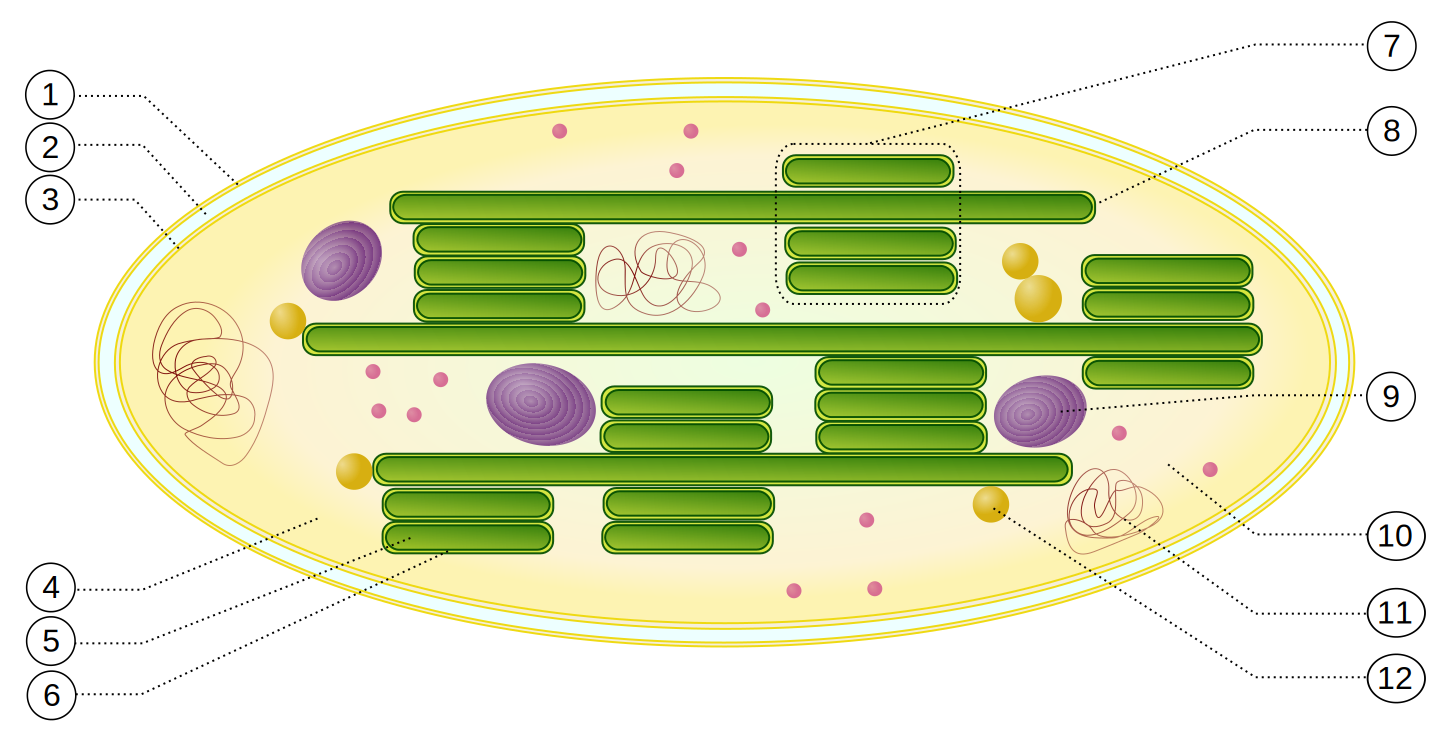
\includegraphics[width=0.7\linewidth]{./figures/photosynthesis/Chloroplast} 

}

\caption{\href{https://commons.wikimedia.org/wiki/File:Chloroplast.svg}{Chloroplast ultrastructure}: 1. outer membrane 2. intermembrane space 3. inner membrane (1+2+3: envelope) 4. stroma (aqueous fluid) 5. thylakoid lumen (inside of thylakoid) 6. thylakoid membrane 7. granum (stack of thylakoids) 8. thylakoid (lamella) 9. starch 10. ribosome 11. plastidial DNA 12. plastoglobule (drop of lipids)}\label{fig:photochloroplast}
\end{figure}

Plants absorb light primarily using the pigment chlorophyll. The green part of the light spectrum is not absorbed but is reflected which is the reason that most plants have a green color. Besides chlorophyll, plants also use pigments such as carotenes and xanthophylls. Algae also use chlorophyll, but various other pigments are present, such as phycocyanin, carotenes, and xanthophylls in green algae, phycoerythrin in red algae (rhodophytes) and fucoxanthin in brown algae and diatoms resulting in a wide variety of colors.

These pigments are embedded in plants and algae in complexes called antenna proteins. In such proteins, the pigments are arranged to work together. Such a combination of proteins is also called a light-harvesting complex.

Although all cells in the green parts of a plant have chloroplasts, the majority of those are found in specially adapted structures called leaves. Certain species adapted to conditions of strong sunlight and aridity, such as many Euphorbia and cactus species, have their main photosynthetic organs in their stems. The cells in the interior tissues of a leaf, called the mesophyll, can contain between 450,000 and 800,000 chloroplasts for every square millimeter of leaf. The surface of the leaf is coated with a water-resistant waxy cuticle that protects the leaf from excessive evaporation of water and decreases the absorption of ultraviolet or blue light to reduce heating. The transparent epidermis layer allows light to pass through to the palisade mesophyll cells where most of the photosynthesis takes place.

In the light-dependent reactions, one molecule of the pigment chlorophyll absorbs one photon and loses one electron. This electron is passed to a modified form of chlorophyll called pheophytin, which passes the electron to a quinone molecule, starting the flow of electrons down an electron transport chain that leads to the ultimate reduction of NADP to NADPH. In addition, this creates a proton gradient (energy gradient) across the chloroplast membrane, which is used by ATP synthase in the synthesis of ATP. The chlorophyll molecule ultimately regains the electron it lost when a water molecule is split in a process called photolysis, which releases a dioxygen (O\textsubscript{2}) molecule as a waste product.

The overall equation for the light-dependent reactions under the conditions of non-cyclic electron flow in green plants is:

2 H\textsubscript{2}O + 2 NADP\textsuperscript{+} + 3 ADP + 3 P\textsubscript{i} + light → 2 NADPH + 2 H\textsubscript{+} + 3 ATP + O\textsubscript{2}

Not all wavelengths of light can support photosynthesis. The photosynthetic action spectrum depends on the type of accessory pigments present. For example, in green plants, the action spectrum resembles the absorption spectrum for chlorophylls and carotenoids with absorption peaks in violet-blue and red light. In red algae, the action spectrum is blue-green light, which allows these algae to use the blue end of the spectrum to grow in the deeper waters that filter out the longer wavelengths (red light) used by above ground green plants. The non-absorbed part of the light spectrum is what gives photosynthetic organisms their color (e.g., green plants, red algae, purple bacteria) and is the least effective for photosynthesis in the respective organisms.

\hypertarget{z-scheme}{%
\subsection{Z Scheme}\label{z-scheme}}

In plants, light-dependent reactions occur in the thylakoid membranes of the chloroplasts where they drive the synthesis of ATP and NADPH. The light-dependent reactions are of two forms: cyclic and non-cyclic.



\begin{figure}

{\centering 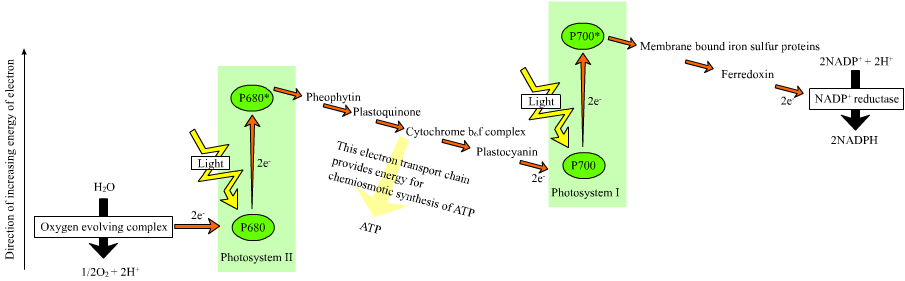
\includegraphics[width=0.7\linewidth]{./figures/photosynthesis/Z-scheme} 

}

\caption{\href{https://commons.wikimedia.org/wiki/File:Z-scheme.png}{The Z scheme}}\label{fig:zscheme}
\end{figure}

In the non-cyclic reaction, the photons are captured in the light-harvesting antenna complexes of photosystem II by chlorophyll and other accessory pigments. The absorption of a photon by the antenna complex frees an electron by a process called photoinduced charge separation. The antenna system is at the core of the chlorophyll molecule of the photosystem II reaction center. That freed electron is transferred to the primary electron-acceptor molecule, pheophytin. As the electrons are shuttled through an electron transport chain (the so-called Z-scheme shown in the diagram), it initially functions to generate a chemiosmotic potential by pumping proton cations (H\textsuperscript{+}) across the membrane and into the thylakoid space. An ATP synthase enzyme uses that chemiosmotic potential to make ATP during photophosphorylation, whereas NADPH is a product of the terminal redox reaction in the Z-scheme. The electron enters a chlorophyll molecule in Photosystem I. There it is further excited by the light absorbed by that photosystem. The electron is then passed along a chain of electron acceptors to which it transfers some of its energy. The energy delivered to the electron acceptors is used to move hydrogen ions across the thylakoid membrane into the lumen. The electron is eventually used to reduce the co-enzyme NADP with a H\textsuperscript{+} to NADPH (which has functions in the light-independent reaction); at that point, the path of that electron ends.



\begin{figure}

{\centering 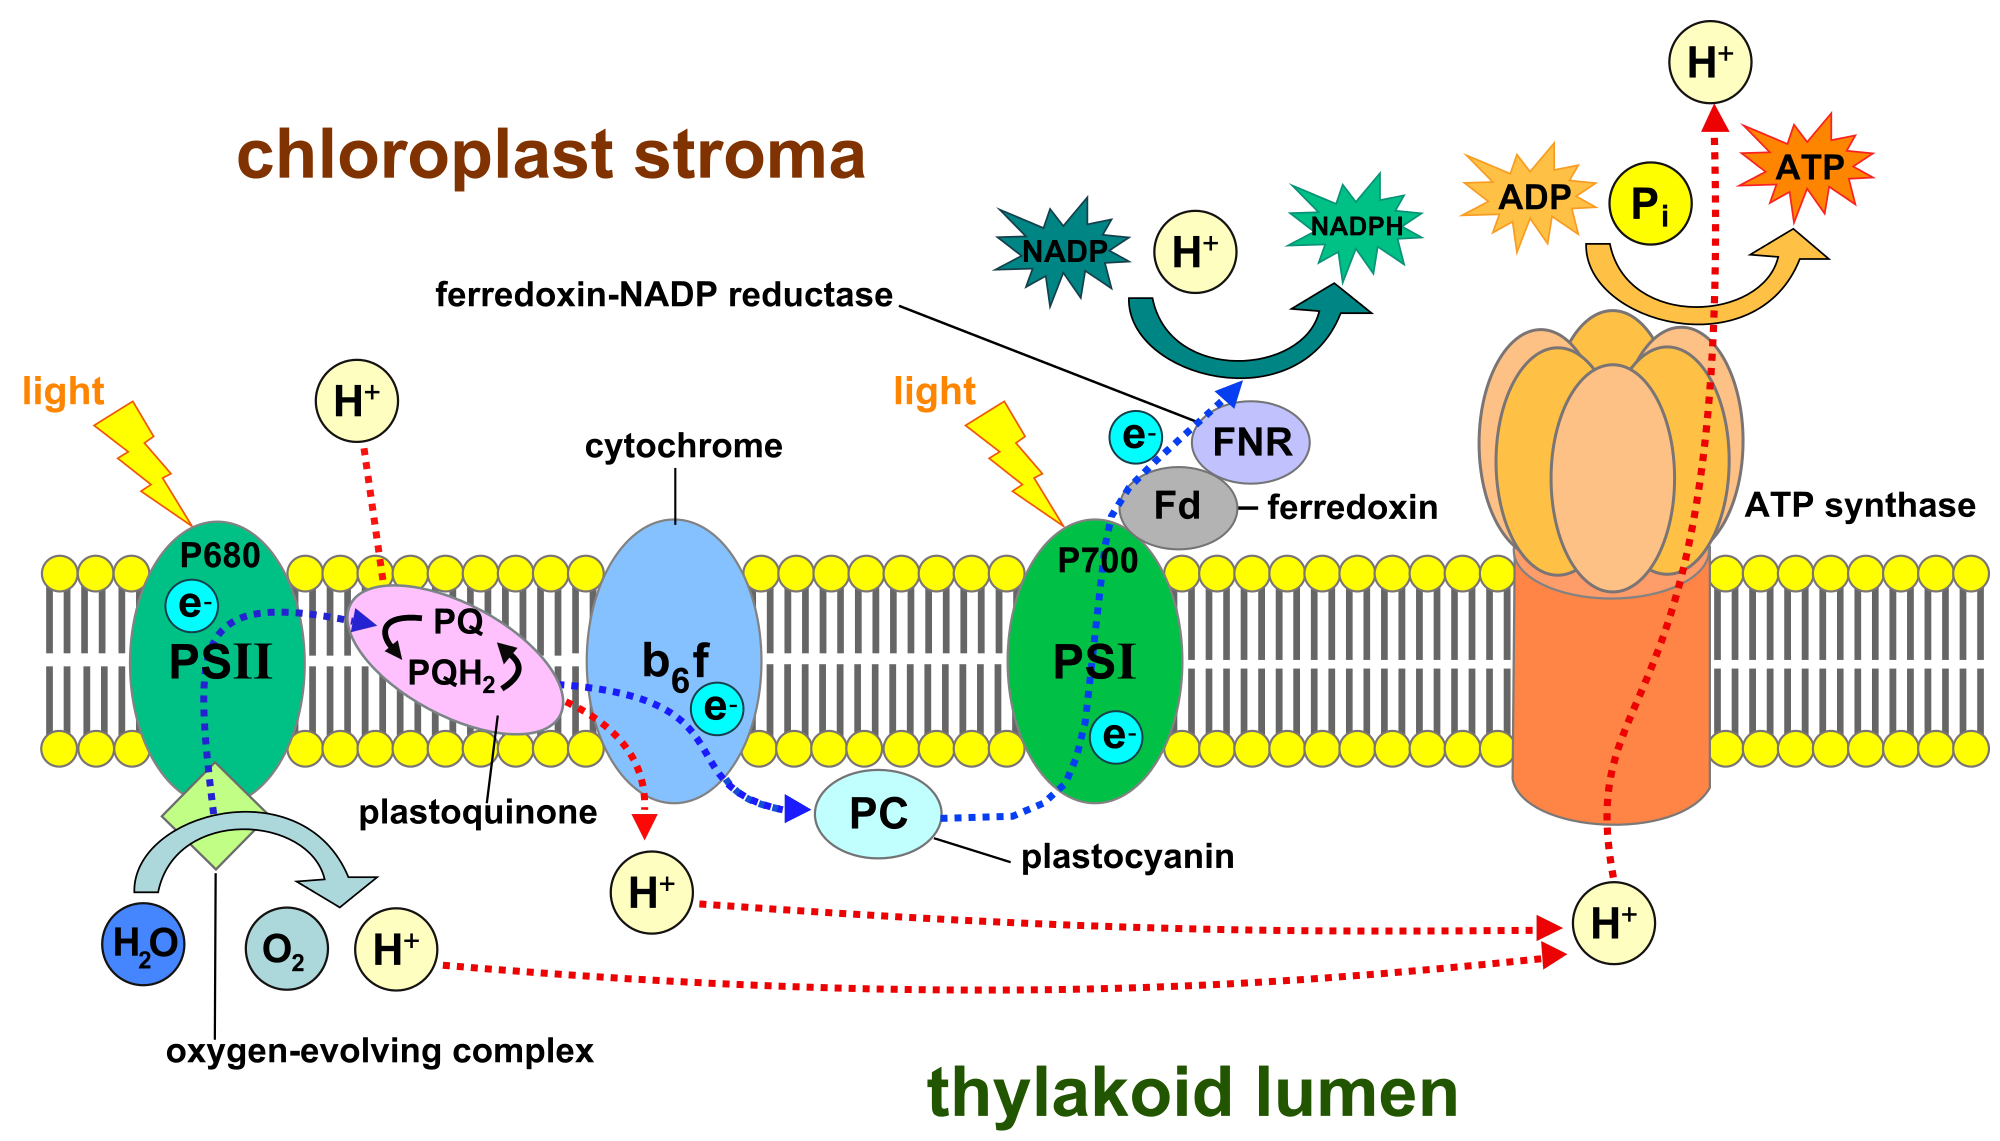
\includegraphics[width=0.7\linewidth]{./figures/photosynthesis/Thylakoid_membrane_3} 

}

\caption{\href{https://commons.wikimedia.org/wiki/File:Thylakoid_membrane_3.svg}{Light-dependent reactions of photosynthesis at the thylakoid membrane}}\label{fig:lightdependent}
\end{figure}

The cyclic reaction is similar to that of the non-cyclic, but differs in that it generates only ATP, and no reduced NADP (NADPH) is created. The cyclic reaction takes place only at photosystem I. Once the electron is displaced from the photosystem, the electron is passed down the electron acceptor molecules and returns to photosystem I, from where it was emitted, hence the name cyclic reaction.

\hypertarget{water-photolysis}{%
\subsection{Water Photolysis}\label{water-photolysis}}

Linear electron transport through a photosystem will leave the reaction center of that photosystem oxidized. Elevating another electron will first require re-reduction of the reaction center. The excited electrons lost from the reaction center (P700) of photosystem I are replaced by transfer from plastocyanin, whose electrons come from electron transport through photosystem II. Photosystem II, as the first step of the Z-scheme, requires an external source of electrons to reduce its oxidized chlorophyll a reaction center, called P680. The source of electrons for photosynthesis in green plants and cyanobacteria is water. Two water molecules are oxidized by four successive charge-separation reactions by photosystem II to yield a molecule of diatomic oxygen and four hydrogen ions. The electrons yielded are transferred to a redox-active tyrosine residue that then reduces the oxidized P680. This resets the ability of P680 to absorb another photon and release another photo-dissociated electron. The oxidation of water is catalyzed in photosystem II by a redox-active structure that contains four manganese ions and a calcium ion; this oxygen-evolving complex binds two water molecules and contains the four oxidizing equivalents that are used to drive the water-oxidizing reaction (Dolai's S-state diagrams). Photosystem II is the only known biological enzyme that carries out this oxidation of water. The hydrogen ions are released in the thylakoid lumen and therefore contribute to the transmembrane chemiosmotic potential that leads to ATP synthesis. Oxygen is a waste product of light-dependent reactions, but the majority of organisms on Earth use oxygen for cellular respiration, including photosynthetic organisms.

\hypertarget{calvin-cycle}{%
\subsection{Calvin Cycle}\label{calvin-cycle}}

In the light-independent (or ``dark'') reactions, the enzyme RuBisCO captures CO\textsubscript{2} from the atmosphere and, in a process called the Calvin cycle, it uses the newly formed NADPH and releases three-carbon sugars, which are later combined to form sucrose and starch. The overall equation for the light-independent reactions in green plants is

3 CO\textsubscript{2} + 9 ATP + 6 NADPH + 6 H\textsuperscript{+} → C\textsubscript{3}H\textsubscript{6}O\textsubscript{3}-phosphate + 9 ADP + 8 P\textsubscript{i} + 6 NADP\textsuperscript{+} + 3 H\textsubscript{2}O

Carbon fixation produces the intermediate three-carbon sugar product, which is then converted into the final carbohydrate products. The simple carbon sugars produced by photosynthesis are then used in the forming of other organic compounds, such as the building material cellulose, the precursors for lipid and amino acid biosynthesis, or as a fuel in cellular respiration. The latter occurs not only in plants but also in animals when the energy from plants is passed through a food chain.



\begin{figure}

{\centering 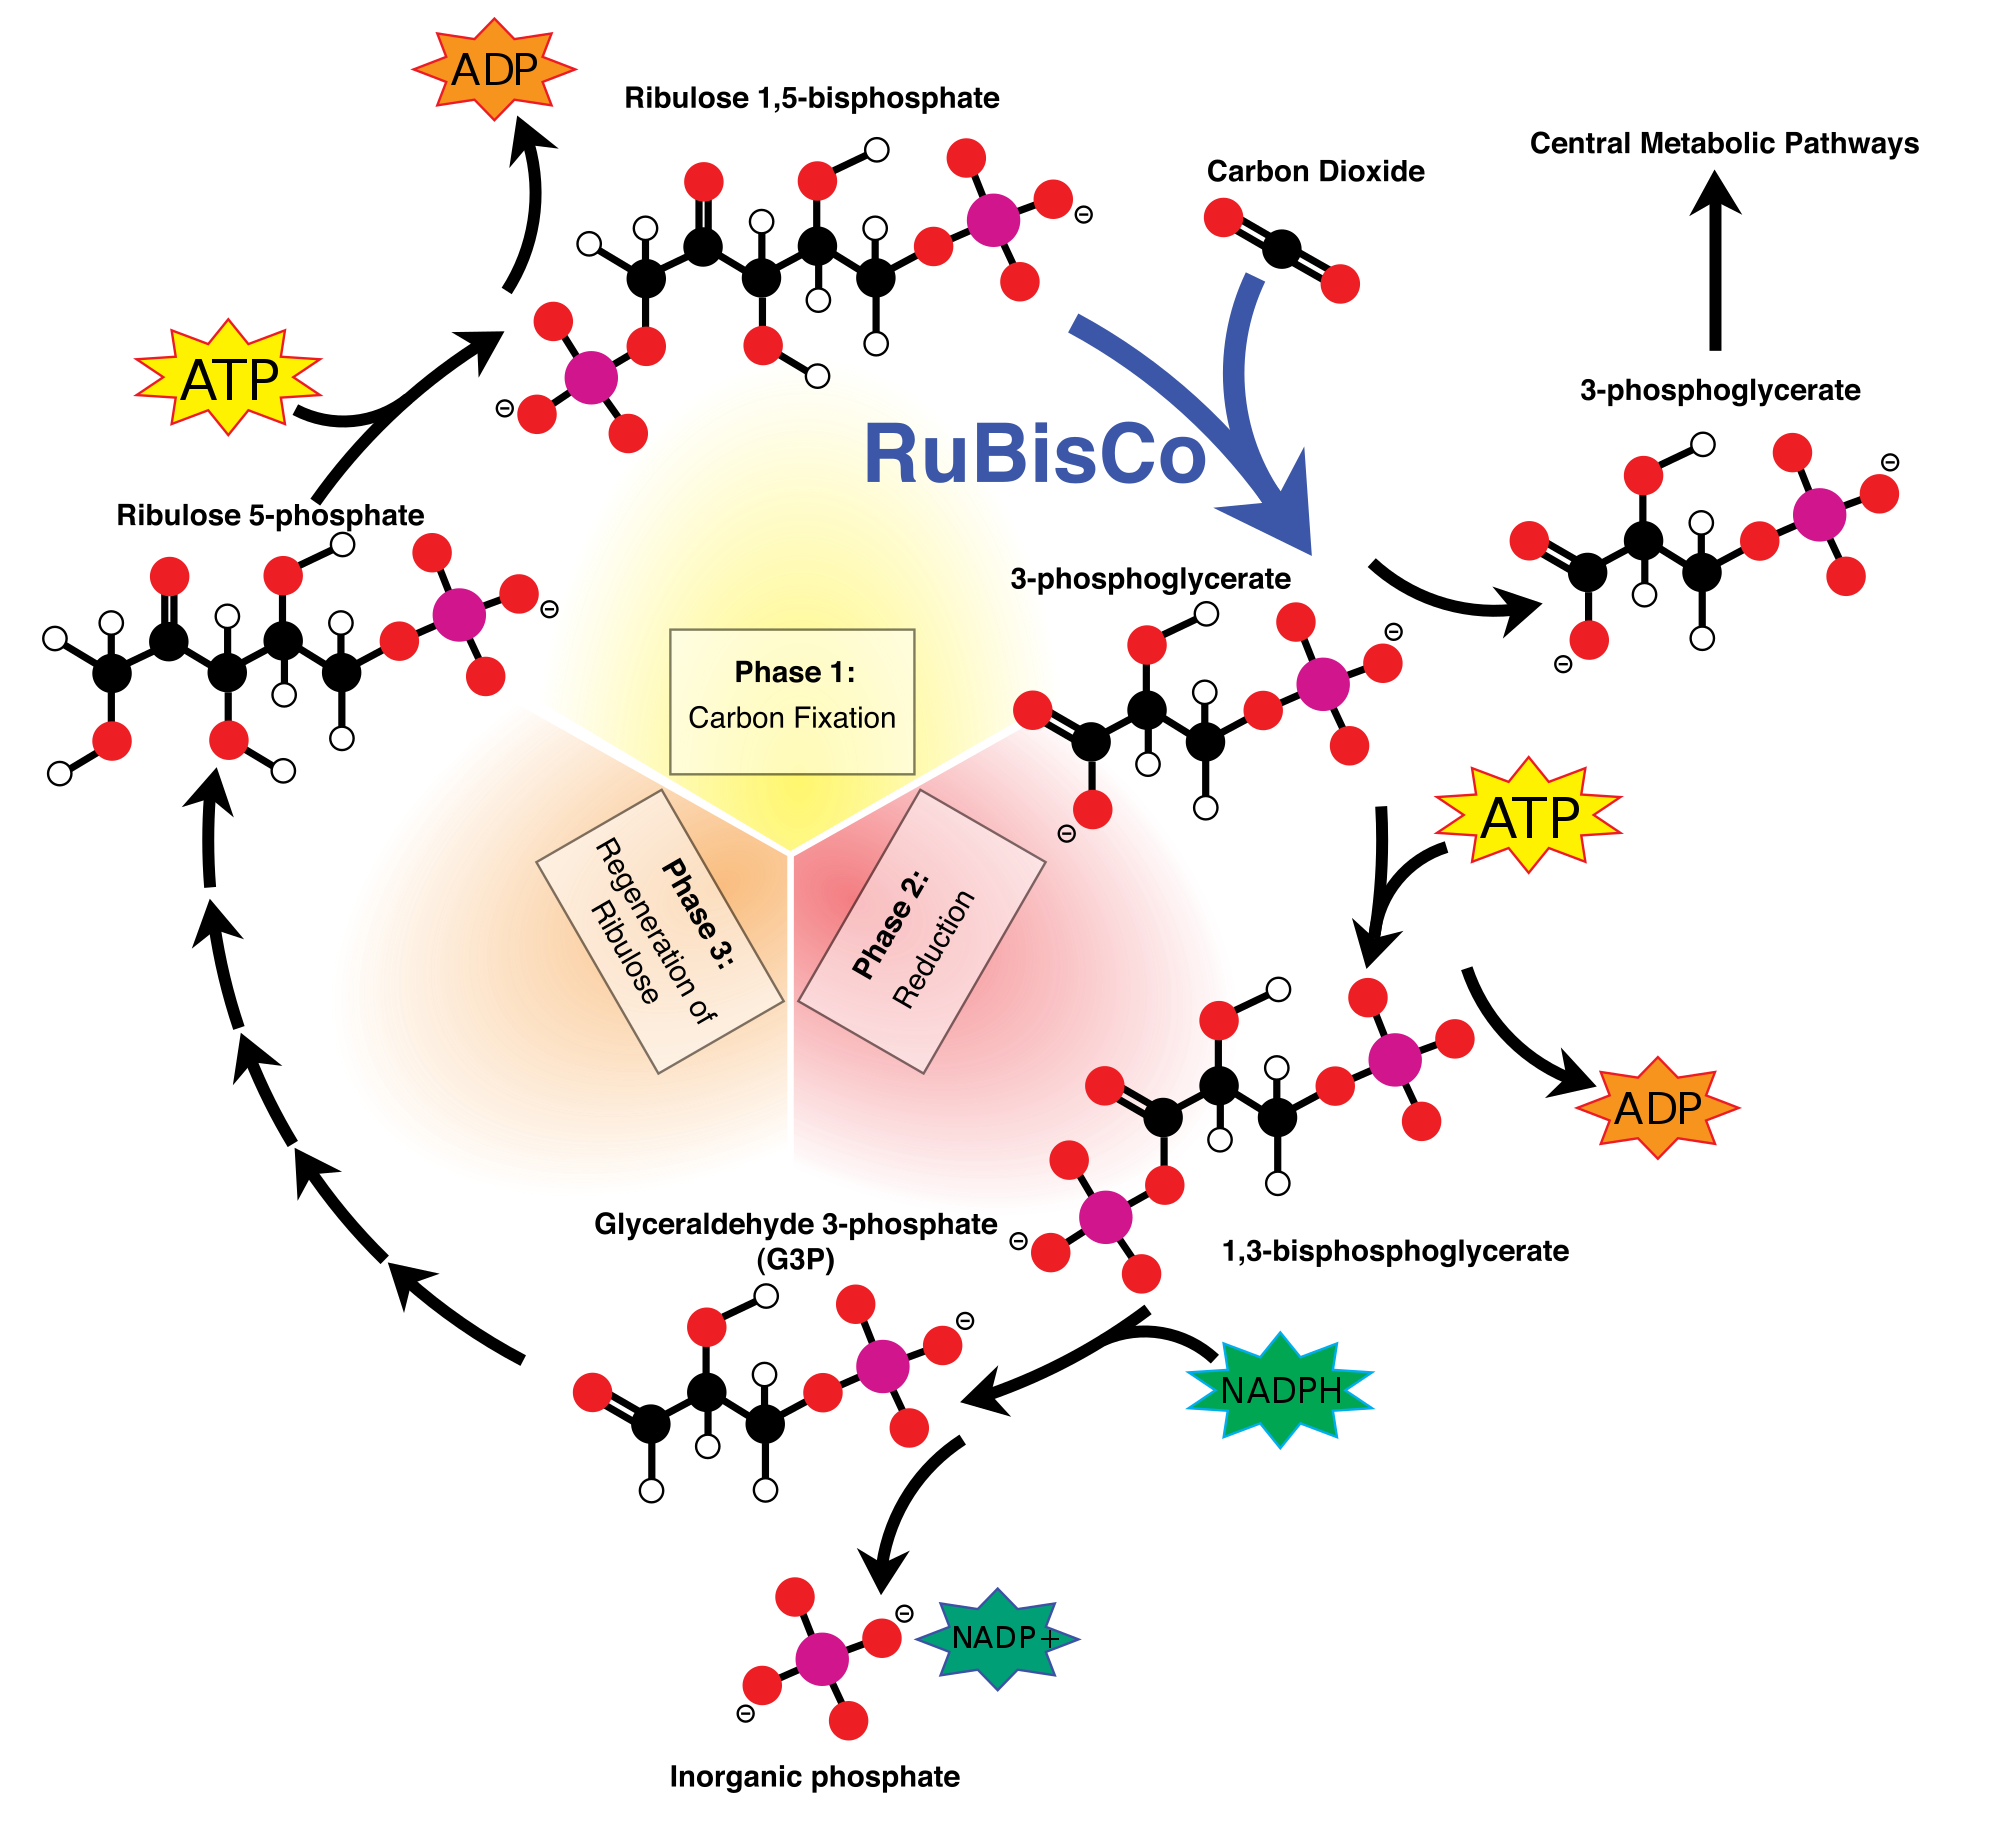
\includegraphics[width=0.7\linewidth]{./figures/photosynthesis/Calvin-cycle4} 

}

\caption{\href{https://commons.wikimedia.org/wiki/File:Calvin-cycle4.svg}{Overview of the Calvin cycle and carbon fixation}}\label{fig:calvincycle}
\end{figure}

The fixation or reduction of carbon dioxide is a process in which carbon dioxide combines with a five-carbon sugar, ribulose 1,5-bisphosphate, to yield two molecules of a three-carbon compound, glycerate 3-phosphate, also known as 3-phosphoglycerate. Glycerate 3-phosphate, in the presence of ATP and NADPH produced during the light-dependent stages, is reduced to glyceraldehyde 3-phosphate. This product is also referred to as 3-phosphoglyceraldehyde (PGAL) or, more generically, as triose phosphate. Most (5 out of 6 molecules) of the glyceraldehyde 3-phosphate produced is used to regenerate ribulose 1,5-bisphosphate so the process can continue. The triose phosphates not thus ``recycled'' often condense to form hexose phosphates, which ultimately yield sucrose, starch and cellulose. The sugars produced during carbon metabolism yield carbon skeletons that can be used for other metabolic reactions like the production of amino acids and lipids.

\hypertarget{carbon-dioxide-levels-and-photorespiration}{%
\subsection{Carbon Dioxide Levels And Photorespiration}\label{carbon-dioxide-levels-and-photorespiration}}

As carbon dioxide concentrations rise, the rate at which sugars are made by the light-independent reactions increases until limited by other factors. RuBisCO, the enzyme that captures carbon dioxide in the light-independent reactions, has a binding affinity for both carbon dioxide and oxygen. When the concentration of carbon dioxide is high, RuBisCO will fix carbon dioxide. However, if the carbon dioxide concentration is low, RuBisCO will bind oxygen instead of carbon dioxide. This process, called photorespiration, uses energy, but does not produce sugars.

RuBisCO oxygenase activity is disadvantageous to plants for several reasons:

\begin{enumerate}
\def\labelenumi{\arabic{enumi}.}
\tightlist
\item
  One product of oxygenase activity is phosphoglycolate (2 carbon) instead of 3-phosphoglycerate (3 carbon). Phosphoglycolate cannot be metabolized by the Calvin-Benson cycle and represents carbon lost from the cycle. A high oxygenase activity, therefore, drains the sugars that are required to recycle ribulose 5-bisphosphate and for the continuation of the Calvin-Benson cycle.
\item
  Phosphoglycolate is quickly metabolized to glycolate that is toxic to a plant at a high concentration; it inhibits photosynthesis.
\item
  Salvaging glycolate is an energetically expensive process that uses the glycolate pathway, and only 75\% of the carbon is returned to the Calvin-Benson cycle as 3-phosphoglycerate. The reactions also produce ammonia (NH\textsubscript{3}), which is able to diffuse out of the plant, leading to a loss of nitrogen.
  A highly simplified summary is:
\end{enumerate}

2 glycolate + ATP → 3-phosphoglycerate + carbon dioxide + ADP + NH\textsubscript{3}

The salvaging pathway for the products of RuBisCO oxygenase activity is more commonly known as photorespiration, since it is characterized by light-dependent oxygen consumption and the release of carbon dioxide.



\begin{figure}

{\centering 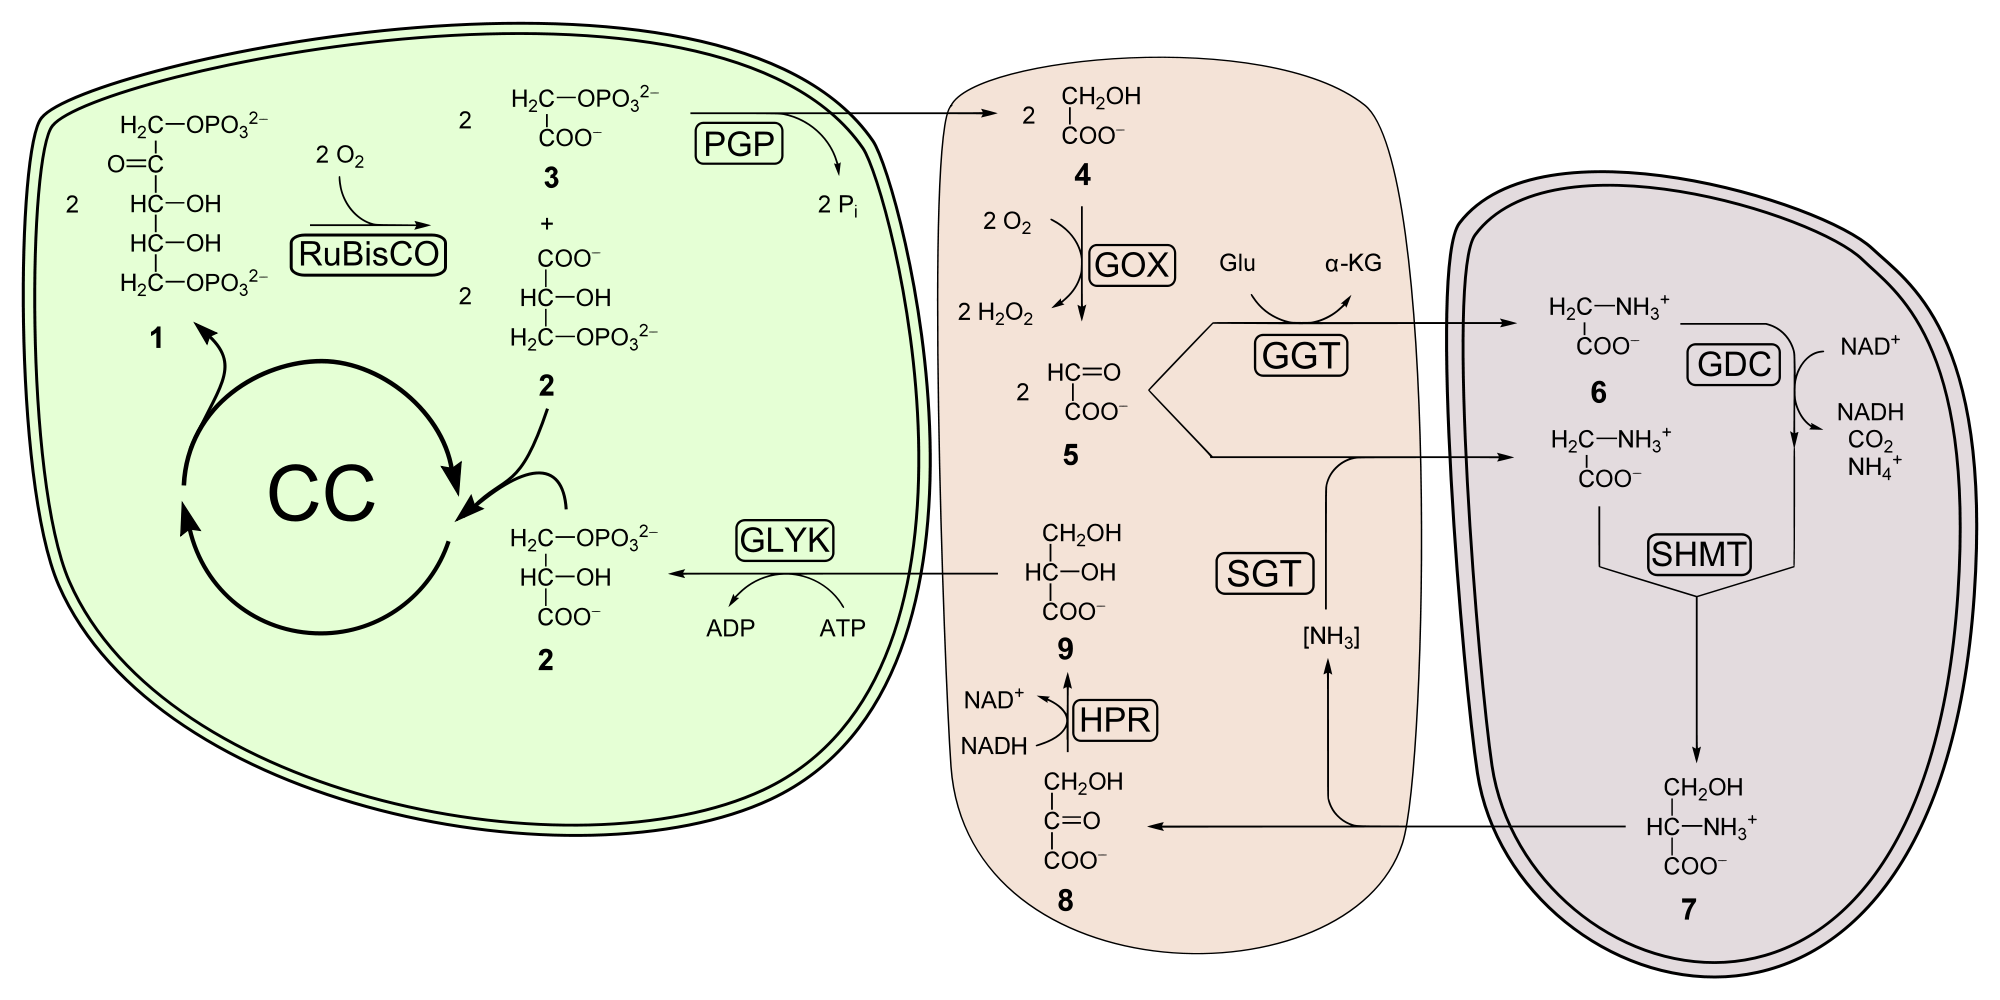
\includegraphics[width=0.7\linewidth]{./figures/photosynthesis/Photorespiration} 

}

\caption{\href{https://commons.wikimedia.org/wiki/File:Photorespiration.svg}{Photorespiration} 1. ribulose 1,5-bisphosphate 2. 3-Phosphoglycerate 3. 2-phosphoglycolate 4. glycolate 5. glyoxylate 6. glycine 7. serine 8. hydroxypyruvate 9. glycerate CC Calvin cycle}\label{fig:photorespiration}
\end{figure}

\hypertarget{c4-carbon-fixation}{%
\subsection{C4 Carbon Fixation}\label{c4-carbon-fixation}}

In hot and dry conditions, plants close their stomata to prevent water loss. Under these conditions, CO\textsubscript{2} will decrease and oxygen gas, produced by the light reactions of photosynthesis, will increase, causing an increase of photorespiration by the oxygenase activity of ribulose-1,5-bisphosphate carboxylase/oxygenase and decrease in carbon fixation. Some plants have evolved mechanisms to increase the CO\textsubscript{2} concentration in the leaves under these conditions.



\begin{figure}

{\centering \includegraphics[width=0.7\linewidth]{./figures/photosynthesis/HatchSlackpathway2} 

}

\caption{\href{https://commons.wikimedia.org/wiki/File:HatchSlackpathway2.svg}{Overview of C4 carbon fixation}}\label{fig:c4carbon}
\end{figure}

Plants that use the C4 carbon fixation process chemically fix carbon dioxide in the cells of the mesophyll by adding it to the three-carbon molecule phosphoenolpyruvate (PEP), a reaction catalyzed by an enzyme called PEP carboxylase, creating the four-carbon organic acid oxaloacetic acid. Oxaloacetic acid or malate synthesized by this process is then translocated to specialized bundle sheath cells where the enzyme RuBisCO and other Calvin cycle enzymes are located, and where CO\textsubscript{2} released by decarboxylation of the four-carbon acids is then fixed by RuBisCO activity to the three-carbon 3-phosphoglyceric acids. The physical separation of RuBisCO from the oxygen-generating light reactions reduces photorespiration and increases CO\textsubscript{2} fixation and, thus, the photosynthetic capacity of the leaf. C4 plants can produce more sugar than C3 plants in conditions of high light and temperature. Many important crop plants are C4 plants, including maize, sorghum, sugarcane, and millet. Plants that do not use PEP-carboxylase in carbon fixation are called C3 plants because the primary carboxylation reaction, catalyzed by RuBisCO, produces the three-carbon 3-phosphoglyceric acids directly in the Calvin-Benson cycle. Over 90\% of plants use C3 carbon fixation, compared to 3\% that use C4 carbon fixation; however, the evolution of C4 in over 60 plant lineages makes it a striking example of convergent evolution.

\hypertarget{cam-photosynthesis}{%
\subsection{CAM Photosynthesis}\label{cam-photosynthesis}}

Xerophytes, such as cacti and most succulents, also use PEP carboxylase to capture carbon dioxide in a process called Crassulacean acid metabolism (CAM). In contrast to C4 metabolism, which spatially separates the CO
2 fixation to PEP from the Calvin cycle, CAM temporally separates these two processes. CAM plants have a different leaf anatomy from C3 plants, and fix the CO\textsubscript{2} at night, when their stomata are open. CAM plants store the CO\textsubscript{2} mostly in the form of malic acid via carboxylation of phosphoenolpyruvate to oxaloacetate, which is then reduced to malate. Decarboxylation of malate during the day releases CO\textsubscript{2} inside the leaves, thus allowing carbon fixation to 3-phosphoglycerate by RuBisCO. Sixteen thousand species of plants use CAM.

Early photosynthetic systems, such as those in green and purple sulfur and green and purple nonsulfur bacteria, are thought to have been anoxygenic, and used various other molecules than water as electron donors. Green and purple sulfur bacteria are thought to have used hydrogen and sulfur as electron donors. Green nonsulfur bacteria used various amino and other organic acids as an electron donor. Purple nonsulfur bacteria used a variety of nonspecific organic molecules. The use of these molecules is consistent with the geological evidence that Earth's early atmosphere was highly reducing at that time.

Fossils of what are thought to be filamentous photosynthetic organisms have been dated at 3.4 billion years old. More recent studies, reported in March 2018, also suggest that photosynthesis may have begun about 3.4 billion years ago.

The main source of oxygen in the Earth's atmosphere derives from oxygenic photosynthesis, and its first appearance is sometimes referred to as the oxygen catastrophe. Geological evidence suggests that oxygenic photosynthesis, such as that in cyanobacteria, became important during the Paleoproterozoic era around 2 billion years ago. Modern photosynthesis in plants and most photosynthetic prokaryotes is oxygenic. Oxygenic photosynthesis uses water as an electron donor, which is oxidized to molecular oxygen (O\textsubscript{2}) in the photosynthetic reaction center.

\hypertarget{symbiosis-and-the-origin-of-chloroplasts}{%
\section{Symbiosis And The Origin of Chloroplasts}\label{symbiosis-and-the-origin-of-chloroplasts}}

Several groups of animals have formed symbiotic relationships with photosynthetic algae. These are most common in corals, sponges and sea anemones. It is presumed that this is due to the particularly simple body plans and large surface areas of these animals compared to their volumes. In addition, a few marine mollusks \emph{Elysia viridis} and \emph{Elysia chlorotica} also maintain a symbiotic relationship with chloroplasts they capture from the algae in their diet and then store in their bodies (see Kleptoplasty). This allows the mollusks to survive solely by photosynthesis for several months at a time. Some of the genes from the plant cell nucleus have even been transferred to the slugs, so that the chloroplasts can be supplied with proteins that they need to survive.

An even closer form of symbiosis may explain the origin of chloroplasts. Chloroplasts have many similarities with photosynthetic bacteria, including a circular chromosome, prokaryotic-type ribosome, and similar proteins in the photosynthetic reaction center. The endosymbiotic theory suggests that photosynthetic bacteria were acquired (by endocytosis) by early eukaryotic cells to form the first plant cells. Therefore, chloroplasts may be photosynthetic bacteria that adapted to life inside plant cells. Like mitochondria, chloroplasts possess their own DNA, separate from the nuclear DNA of their plant host cells and the genes in this chloroplast DNA resemble those found in cyanobacteria. DNA in chloroplasts codes for redox proteins such as those found in the photosynthetic reaction centers. The CoRR Hypothesis proposes that this co-location of genes with their gene products is required for redox regulation of gene expression, and accounts for the persistence of DNA in bioenergetic organelles.

\hypertarget{cyanobacteria-and-the-evolution-of-photosynthesis}{%
\section{Cyanobacteria And The Evolution of Photosynthesis}\label{cyanobacteria-and-the-evolution-of-photosynthesis}}

The biochemical capacity to use water as the source for electrons in photosynthesis evolved once, in a common ancestor of extant cyanobacteria (formerly called blue-green algae), which are the only prokaryotes performing oxygenic photosynthesis. The geological record indicates that this transforming event took place early in Earth's history, at least 2450--2320 million years ago (Ma), and, it is speculated, much earlier. Because the Earth's atmosphere contained almost no oxygen during the estimated development of photosynthesis, it is believed that the first photosynthetic cyanobacteria did not generate oxygen. Available evidence from geobiological studies of Archean (\textgreater2500 Ma) sedimentary rocks indicates that life existed 3500 Ma, but the question of when oxygenic photosynthesis evolved is still unanswered. A clear paleontological window on cyanobacterial evolution opened about 2000 Ma, revealing an already-diverse biota of Cyanobacteria. Cyanobacteria remained the principal primary producers of oxygen throughout the Proterozoic Eon (2500--543 Ma), in part because the redox structure of the oceans favored photoautotrophs capable of nitrogen fixation. Green algae joined cyanobacteria as the major primary producers of oxygen on continental shelves near the end of the Proterozoic, but it was only with the Mesozoic (251--66 Ma) radiations of dinoflagellates, coccolithophorids, and diatoms did the primary production of oxygen in marine shelf waters take modern form. Cyanobacteria remain critical to marine ecosystems as primary producers of oxygen in oceanic gyres, as agents of biological nitrogen fixation, and, in modified form, as the plastids of marine algae.

\hypertarget{cellular-respiration}{%
\section{Cellular Respiration}\label{cellular-respiration}}

Cellular respiration is a set of metabolic reactions and processes that take place in the cells of organisms to convert chemical energy from oxygen molecules or nutrients into adenosine triphosphate (ATP), and then release waste products. The reactions involved in respiration are catabolic reactions, which break large molecules into smaller ones, releasing energy because weak high-energy bonds, in particular in molecular oxygen, are replaced by stronger bonds in the products. Respiration is one of the key ways a cell releases chemical energy to fuel cellular activity. The overall reaction occurs in a series of biochemical steps, some of which are redox reactions. Although cellular respiration is technically a combustion reaction, it clearly does not resemble one when it occurs in a living cell because of the slow, controlled release of energy from the series of reactions.



\begin{figure}

{\centering \includegraphics[width=0.7\linewidth]{./figures/photosynthesis/CellRespiration} 

}

\caption{\href{https://commons.wikimedia.org/wiki/File:CellRespiration.svg}{A diagram of cellular respiration including glycolysis, Krebs cycle (AKA citric acid cycle), and the electron transport chain}}\label{fig:cellularrespiration}
\end{figure}

Nutrients that are commonly used by animal and plant cells in respiration include sugar, amino acids and fatty acids, and the most common oxidizing agent providing most of the chemical energy is molecular oxygen (O\textsubscript{2}). The chemical energy stored in ATP (the bond of its third phosphate group to the rest of the molecule can be broken allowing more stable products to form, thereby releasing energy for use by the cell) can then be used to drive processes requiring energy, including biosynthesis, locomotion or transport of molecules across cell membranes.

\hypertarget{aerobic-respiration}{%
\subsection{Aerobic Respiration}\label{aerobic-respiration}}

Aerobic respiration requires oxygen (O\textsubscript{2}) in order to create ATP. Although carbohydrates, fats, and proteins are consumed as reactants, aerobic respiration is the preferred method of pyruvate breakdown in glycolysis, and requires pyruvate to the mitochondria in order to be fully oxidized by the citric acid cycle. The products of this process are carbon dioxide and water, and the energy transferred is used to break bonds in ADP to add a third phosphate group to form ATP (adenosine triphosphate), by substrate-level phosphorylation, NADH and FADH2

Simplified reaction:

C\textsubscript{6}H\textsubscript{12}O\textsubscript{6} (s) + 6 O\textsubscript{2} (g) → 6 CO\textsubscript{2} (g) + 6 H\textsubscript{2}O (l) + heat

ΔG = −2880 kJ per mol of C\textsubscript{6}H\textsubscript{12}O\textsubscript{6}

The negative ΔG indicates that the reaction can occur spontaneously.

The potential of NADH and FADH\textsubscript{2} is converted to more ATP through an electron transport chain with oxygen and protons (hydrogen) as the ``terminal electron acceptors''. Most of the ATP produced by aerobic cellular respiration is made by oxidative phosphorylation. The energy of O\textsubscript{2} released is used to create a chemiosmotic potential by pumping protons across a membrane. This potential is then used to drive ATP synthase and produce ATP from ADP and a phosphate group. Biology textbooks often state that 38 ATP molecules can be made per oxidized glucose molecule during cellular respiration (2 from glycolysis, 2 from the Krebs cycle, and about 34 from the electron transport system). However, this maximum yield is never quite reached because of losses due to leaky membranes as well as the cost of moving pyruvate and ADP into the mitochondrial matrix, and current estimates range around 29 to 30 ATP per glucose.



\begin{figure}

{\centering 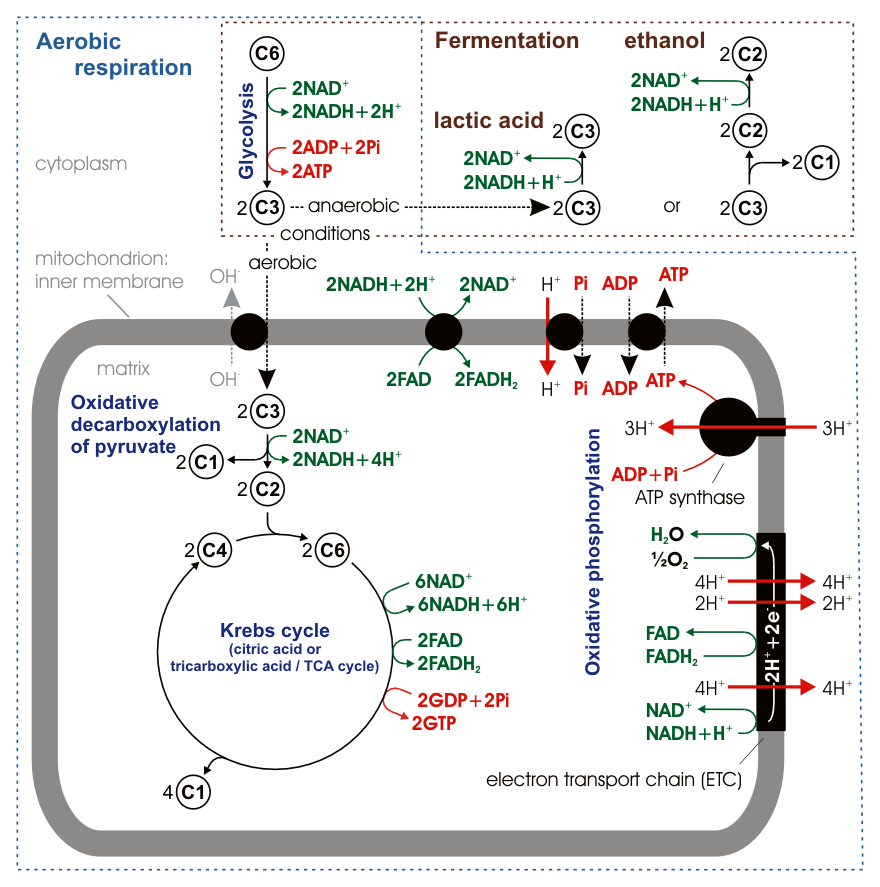
\includegraphics[width=0.7\linewidth]{./figures/photosynthesis/Cellular_respiration} 

}

\caption{\href{https://commons.wikimedia.org/wiki/File:Cellular_respiration.gif}{Stoichiometry of aerobic respiration} and most known fermentation types in eucaryotic cell. Numbers in circles indicate counts of carbon atoms in molecules, C6 is glucose C\textsubscript{6}H\textsubscript{12}O\textsubscript{6}, C1 carbon dioxide CO\textsubscript{2}. Mitochondrial outer membrane is omitted.}\label{fig:cellresstoich}
\end{figure}

Aerobic metabolism is up to 15 times more efficient than anaerobic metabolism (which yields 2 molecules ATP per 1 molecule glucose) because the double bond in O\textsubscript{2} is of higher energy than other double bonds or pairs of single bonds in other common molecules in the biosphere. However, some anaerobic organisms, such as methanogens are able to continue with anaerobic respiration, yielding more ATP by using other inorganic molecules (not oxygen) of high energy as final electron acceptors in the electron transport chain. They share the initial pathway of glycolysis but aerobic metabolism continues with the Krebs cycle and oxidative phosphorylation. The post-glycolytic reactions take place in the mitochondria in eukaryotic cells, and in the cytoplasm in prokaryotic cells.

\hypertarget{glycolysis}{%
\subsection{Glycolysis}\label{glycolysis}}

Out of the cytoplasm it goes into the Krebs cycle with the acetyl CoA. It then mixes with CO\textsubscript{2} and makes 2 ATP, NADH, and FADH. From there the NADH and FADH go into the NADH reductase, which produces the enzyme. The NADH pulls the enzyme's electrons to send through the electron transport chain. The electron transport chain pulls H\textsuperscript{+} ions through the chain. From the electron transport chain, the released hydrogen ions make ADP for an end result of 32 ATP. O\textsubscript{2} provides most of the energy for the process and combines with protons and the electrons to make water. Lastly, ATP leaves through the ATP channel and out of the mitochondria.
Main article: Glycolysis
Glycolysis is a metabolic pathway that takes place in the cytosol of cells in all living organisms. Glycolysis can be literally translated as ``sugar splitting'', and occurs with or without the presence of oxygen. In aerobic conditions, the process converts one molecule of glucose into two molecules of pyruvate (pyruvic acid), generating energy in the form of two net molecules of ATP. Four molecules of ATP per glucose are actually produced, however, two are consumed as part of the preparatory phase. The initial phosphorylation of glucose is required to increase the reactivity (decrease its stability) in order for the molecule to be cleaved into two pyruvate molecules by the enzyme aldolase. During the pay-off phase of glycolysis, four phosphate groups are transferred to ADP by substrate-level phosphorylation to make four ATP, and two NADH are produced when the pyruvate is oxidized. The overall reaction can be expressed this way:

Glucose + 2 NAD\textsuperscript{+} + 2 P\textsubscript{i} + 2 ADP → 2 pyruvate + 2 H\textsuperscript{+} + 2 NADH + 2 ATP + 2 H\textsuperscript{+} + 2 H\textsubscript{2}O + energy

Starting with glucose, 1 ATP is used to donate a phosphate to glucose to produce glucose 6-phosphate. Glycogen can be converted into glucose 6-phosphate as well with the help of glycogen phosphorylase. During energy metabolism, glucose 6-phosphate becomes fructose 6-phosphate. An additional ATP is used to phosphorylate fructose 6-phosphate into fructose 1,6-bisphosphate by the help of phosphofructokinase. Fructose 1,6-biphosphate then splits into two phosphorylated molecules with three carbon chains which later degrades into pyruvate.

\hypertarget{oxidative-decarboxylation-of-pyruvate}{%
\subsection{Oxidative Decarboxylation of Pyruvate}\label{oxidative-decarboxylation-of-pyruvate}}

Pyruvate is oxidized to acetyl-CoA and CO\textsubscript{2} by the pyruvate dehydrogenase complex (PDC). The PDC contains multiple copies of three enzymes and is located in the mitochondria of eukaryotic cells and in the cytosol of prokaryotes. In the conversion of pyruvate to acetyl-CoA, one molecule of NADH and one molecule of CO\textsubscript{2} is formed.

\hypertarget{the-citric-acid-cycle}{%
\subsection{The Citric Acid Cycle}\label{the-citric-acid-cycle}}

This is also called the Krebs cycle or the tricarboxylic acid cycle. When oxygen is present, acetyl-CoA is produced from the pyruvate molecules created from glycolysis. Once acetyl-CoA is formed, aerobic or anaerobic respiration can occur. When oxygen is present, the mitochondria will undergo aerobic respiration which leads to the Krebs cycle. However, if oxygen is not present, fermentation of the pyruvate molecule will occur. In the presence of oxygen, when acetyl-CoA is produced, the molecule then enters the citric acid cycle (Krebs cycle) inside the mitochondrial matrix, and is oxidized to CO\textsubscript{2} while at the same time reducing NAD to NADH. NADH can be used by the electron transport chain to create further ATP as part of oxidative phosphorylation. To fully oxidize the equivalent of one glucose molecule, two acetyl-CoA must be metabolized by the Krebs cycle. Two low-energy waste products, H\textsubscript{2}O and CO\textsubscript{2}, are created during this cycle.

The citric acid cycle is an 8-step process involving 18 different enzymes and co-enzymes. During the cycle, acetyl-CoA (2 carbons) + oxaloacetate (4 carbons) yields citrate (6 carbons), which is rearranged to a more reactive form called isocitrate (6 carbons). Isocitrate is modified to become α-ketoglutarate (5 carbons), succinyl-CoA, succinate, fumarate, malate, and, finally, oxaloacetate.

The net gain from one cycle is 3 NADH and 1 FADH2 as hydrogen- (proton plus electron)-carrying compounds and 1 high-energy GTP, which may subsequently be used to produce ATP. Thus, the total yield from 1 glucose molecule (2 pyruvate molecules) is 6 NADH, 2 FADH\textsubscript{2}, and 2 ATP.

\hypertarget{oxidative-phosphorylation-1}{%
\subsection{Oxidative Phosphorylation}\label{oxidative-phosphorylation-1}}

In eukaryotes, oxidative phosphorylation occurs in the mitochondrial cristae. It comprises the electron transport chain that establishes a proton gradient (chemiosmotic potential) across the boundary of the inner membrane by oxidizing the NADH produced from the Krebs cycle. ATP is synthesized by the ATP synthase enzyme when the chemiosmotic gradient is used to drive the phosphorylation of ADP. The electron transfer is driven by the chemical energy of exogenous oxygen and, with the addition of two protons, water is formed.

\hypertarget{fermentation}{%
\section{Fermentation}\label{fermentation}}

Without oxygen, pyruvate (pyruvic acid) is not metabolized by cellular respiration but undergoes a process of fermentation. The pyruvate is not transported into the mitochondrion, but remains in the cytoplasm, where it is converted to waste products that may be removed from the cell. This serves the purpose of oxidizing the electron carriers so that they can perform glycolysis again and removing the excess pyruvate. Fermentation oxidizes NADH to NAD\textsuperscript{+} so it can be re-used in glycolysis. In the absence of oxygen, fermentation prevents the buildup of NADH in the cytoplasm and provides NAD\textsuperscript{+} for glycolysis. This waste product varies depending on the organism. In skeletal muscles, the waste product is lactic acid. This type of fermentation is called lactic acid fermentation. In strenuous exercise, when energy demands exceed energy supply, the respiratory chain cannot process all of the hydrogen atoms joined by NADH. During anaerobic glycolysis, NAD\textsuperscript{+} regenerates when pairs of hydrogen combine with pyruvate to form lactate. Lactate formation is catalyzed by lactate dehydrogenase in a reversible reaction. Lactate can also be used as an indirect precursor for liver glycogen. During recovery, when oxygen becomes available, NAD\textsuperscript{+} attaches to hydrogen from lactate to form ATP. In yeast, the waste products are ethanol and carbon dioxide. This type of fermentation is known as alcoholic or ethanol fermentation. The ATP generated in this process is made by substrate-level phosphorylation, which does not require oxygen.

Fermentation is less efficient at using the energy from glucose: only 2 ATP are produced per glucose, compared to the 38 ATP per glucose nominally produced by aerobic respiration. This is because most of the energy of aerobic respiration derives from O\textsubscript{2} with its relatively weak, high-energy double bond. Glycolytic ATP, however, is created more quickly. For prokaryotes to continue a rapid growth rate when they are shifted from an aerobic environment to an anaerobic environment, they must increase the rate of the glycolytic reactions. For multicellular organisms, during short bursts of strenuous activity, muscle cells use fermentation to supplement the ATP production from the slower aerobic respiration, so fermentation may be used by a cell even before the oxygen levels are depleted, as is the case in sports that do not require athletes to pace themselves, such as sprinting.

Along with photosynthesis and aerobic respiration, fermentation is a way of extracting energy from molecules, but it is the only one common to all bacteria and eukaryotes. It is therefore considered the oldest metabolic pathway, suitable for an environment that did not yet have oxygen. Yeast, a form of fungus, occurs in almost any environment capable of supporting microbes, from the skins of fruits to the guts of insects and mammals and the deep ocean, and harvests sugar-rich materials to produce ethanol and carbon dioxide.

The basic mechanism for fermentation remains present in all cells of higher organisms. Mammalian muscle carries out fermentation during periods of intense exercise where oxygen supply becomes limited, resulting in the creation of lactic acid. In invertebrates, fermentation also produces succinate and alanine.

Fermentative bacteria play an essential role in the production of methane in habitats ranging from the rumens of cattle to sewage digesters and freshwater sediments. They produce hydrogen, carbon dioxide, formate and acetate and carboxylic acids; and then consortia of microbes convert the carbon dioxide and acetate to methane. Acetogenic bacteria oxidize the acids, obtaining more acetate and either hydrogen or formate. Finally, methanogens (in the domain Archea) convert acetate to methane.

In ethanol fermentation, one glucose molecule is converted into two ethanol molecules and two carbon dioxide molecules. It is used to make bread dough rise: the carbon dioxide forms bubbles, expanding the dough into a foam. The ethanol is the intoxicating agent in alcoholic beverages such as wine, beer and liquor. Fermentation of feedstocks, including sugarcane, corn, and sugar beets, produces ethanol that is added to gasoline. In some species of fish, including goldfish and carp, it provides energy when oxygen is scarce (along with lactic acid fermentation).

Before fermentation, a glucose molecule breaks down into two pyruvate molecules (Glycolysis). The energy from this exothermic reaction is used to bind inorganic phosphates to ADP, which converts it to ATP, and convert NAD\textsuperscript{+} to NADH. The pyruvates break down into two acetaldehyde molecules and give off two carbon dioxide molecules as waste products. The acetaldehyde is reduced into ethanol using the energy and hydrogen from NADH, and the NADH is oxidized into NAD\textsuperscript{+} so that the cycle may repeat. The reaction is catalyzed by the enzymes pyruvate decarboxylase and alcohol dehydrogenase.

\hypertarget{anaerobic-respiration}{%
\section{Anaerobic Respiration}\label{anaerobic-respiration}}

Cellular respiration is the process by which biological fuels are oxidised in the presence of a high-energy inorganic electron acceptor (such as oxygen) to produce large amounts of energy, to drive the bulk production of ATP.

Anaerobic respiration is used by some microorganisms in which neither oxygen (aerobic respiration) nor pyruvate derivatives (fermentation) is the high-energy final electron acceptor. Rather, an inorganic acceptor such as sulfate or nitrate is used. Such organisms are typically found in unusual places such as underwater caves or near hydrothermal vents at the bottom of the ocean.

In July 2019, a scientific study of Kidd Mine in Canada discovered sulfur-breathing organisms which live 7900 feet below the surface, and which breathe sulfur in order to survive. These organisms are also remarkable due to consuming minerals such as pyrite as their food source.


